
\subsubsection{16.11.14}

\begin{enumerate} 
	\item The time of beginning and ending of the congregation:
	19:00 - 20:30
	\item Purposes of the congregation:
	\begin{enumerate}
		\item Finish working on the bucket.
		
		\item Fix the bucket at STB.
		
	\end{enumerate}
	
	\item Work, that has been done:
	\begin{enumerate}
		\item Preparation of the bucket was changed: it's top part was was minimized so that the formed pipe. This pipe will roll the balls during tipping the bucket. The bottom part wasn't changed.
		
		\item It was decided fix inside the tube plastic bottle to make the balls easier to slide over the pipe. Today we couldn't make it because we didn't have the bottle.
		
		\item Bucket was fixed at STB.
		
		\item After fixing of bucket to robot it turned out that due to transverse beam in front part of robot bucket can't lowers to maximum bottom position. So that this beam was changed on a more subtle, which doesn't prevent to moving of bucket.
		
	    \begin{figure}[H]
			\begin{minipage}[h]{0.47\linewidth}
				\center{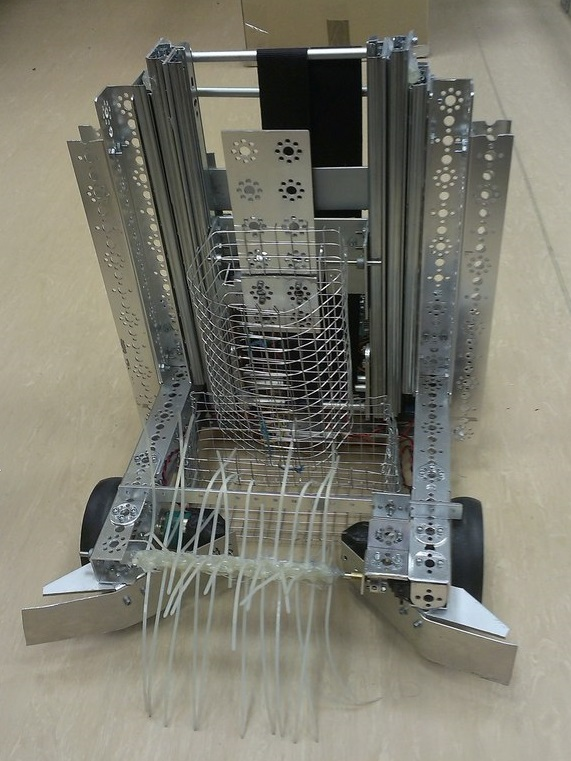
\includegraphics[scale=0.3]{days/16.11.14/images/01}}
				\caption{Bucket in a start position}
			\end{minipage}
			\hfill
			\begin{minipage}[h]{0.47\linewidth}
				\center{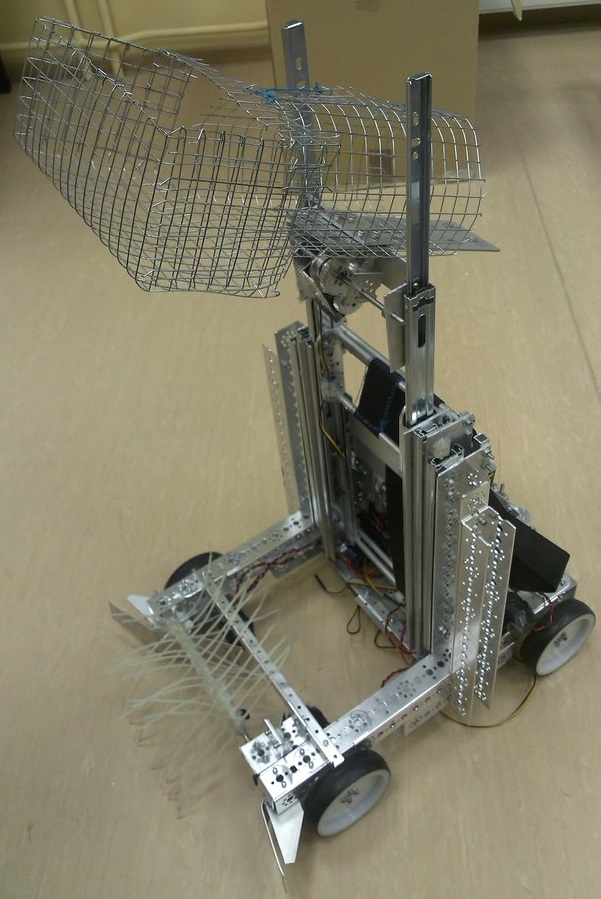
\includegraphics[scale=0.25]{days/16.11.14/images/02}}
				\caption{Bucket in the overturned position}
			\end{minipage}
		\end{figure}
		
	\end{enumerate}
	
	\item Results:
	\begin{enumerate}
		\item Framework of bucket was created and installed to robot.
		
	\end{enumerate}
	
	\item Tasks for the next congregations:
	\begin{enumerate}
		\item Improve the bucket's construction.
		
		\item Test the bucket.
		
	\end{enumerate}     
\end{enumerate}
\fillpage

